\documentclass[10pt,letterpaper]{report}

\usepackage[utf8]{inputenc}
\usepackage[T1]{fontenc}
\usepackage[spanish,es-tabla]{babel}
\usepackage{helvet}
\usepackage{geometry}
\usepackage{graphicx}
\usepackage{float}
\usepackage{longtable}
\usepackage{array}
\usepackage{booktabs}
\usepackage{xcolor}
\usepackage{hyperref}
\usepackage{caption}
\usepackage{enumitem}
\usepackage{setspace}
\usepackage{listings}
\usepackage{fancyvrb}

\renewcommand{\familydefault}{\sfdefault}

\geometry{
  top=20mm,
  bottom=20mm,
  left=25mm,
  right=25mm
}

\setstretch{1.05}
\setlength{\parindent}{0pt}
\setlength{\parskip}{5pt}
\captionsetup{font=small,labelfont=bf}

\definecolor{codegray}{rgb}{0.95,0.95,0.95}
\definecolor{codegreen}{rgb}{0.0,0.5,0.0}
\definecolor{codepurple}{rgb}{0.4,0.0,0.6}
\definecolor{passgreen}{rgb}{0.0,0.55,0.0}

\lstdefinestyle{phpstyle}{
  backgroundcolor=\color{codegray},
  basicstyle=\ttfamily\small,
  keywordstyle=\color{codepurple}\bfseries,
  commentstyle=\color{codegreen},
  stringstyle=\color{orange},
  breaklines=true,
  frame=single,
  rulecolor=\color{gray!40},
  numbers=left,
  numberstyle=\tiny\color{gray},
  numbersep=5pt,
  tabsize=2,
  showstringspaces=false,
  language=PHP
}

\lstdefinestyle{jsstyle}{
  backgroundcolor=\color{codegray},
  basicstyle=\ttfamily\small,
  keywordstyle=\color{codepurple}\bfseries,
  commentstyle=\color{codegreen},
  stringstyle=\color{orange},
  breaklines=true,
  frame=single,
  rulecolor=\color{gray!40},
  numbers=left,
  numberstyle=\tiny\color{gray},
  numbersep=5pt,
  tabsize=2,
  showstringspaces=false
}

\lstdefinestyle{bashstyle}{
  backgroundcolor=\color{codegray},
  basicstyle=\ttfamily\small,
  breaklines=true,
  frame=single,
  rulecolor=\color{gray!40},
  numbers=none,
  tabsize=2,
  showstringspaces=false
}

\hypersetup{
  colorlinks=true,
  linkcolor=black,
  urlcolor=blue,
  pdftitle={Reporte Tecnico - Gestor de Identidades y Documentos MA2006B 2026},
  pdfauthor={Equipo 5}
}

\begin{document}

%%============================================================
%% PORTADA
%%============================================================
\begin{titlepage}
  \centering
  \vspace*{0.5cm}

  {\Large\bfseries Instituto Tecnológico y de Estudios Superiores de Monterrey\par}
  \vspace{0.4cm}
  
\includegraphics[width=0.52\textwidth]{../manual_usuario/logos/tecnologico-de-monterrey-blue.png}
  \vspace{0.5cm}

  {\large\bfseries Escuela de Ingeniería y Ciencias\par}
  \vspace{0.2cm}
  {\large Ingeniería en Ciencia de Datos y Matemáticas\par}
  \vspace{0.2cm}
  {\normalsize Uso de Álgebras Modernas para Seguridad y Criptografía\par}

  \vspace{0.8cm}
  {\Large\bfseries Reporte Técnico\par}
  \vspace{0.2cm}
  {\large Etapa 1 del Reto: Gestor de Identidades y Documentos\par}

  \vspace{0.9cm}
  {\bfseries Socio Formador:} Casa Monarca, Ayuda Humanitaria al Migrante, A.B.P.\par
  \vspace{0.4cm}
  {\bfseries Profesores:} Raúl Gómez, Anas Wajid y Alberto F. Martínez\par

  \vspace{0.7cm}
  {\bfseries Equipo de trabajo:} Equipo 5\par
  {\bfseries Grupo:} 603\par

  \vspace{0.7cm}
  {\bfseries Integrantes}\par
  Alberto Rodríguez Reyes (A01383805)\par
  Diego Alberto Rodríguez Ruiz (A01571638)\par
  Rubén Jiménez Sarmiento (A01286256)\par
  Hector Alonso Flores Meléndez (A01571545)\par
  Valeria García Hernández (A01742811)\par

  \vfill
  {\bfseries Lugar y fecha de elaboración:} Monterrey, Nuevo León, 14 de junio de 2026\par
\end{titlepage}

%%============================================================
%% ÍNDICES
%%============================================================
\pagenumbering{roman}
\tableofcontents
\listoftables
\listoffigures
\clearpage
\pagenumbering{arabic}

%%============================================================
%% ABSTRACT
%%============================================================
\chapter*{Resumen}
\addcontentsline{toc}{chapter}{Resumen}

Este reporte documenta el diseño, implementación y validación del sistema \textbf{Gestor de Identidades y Documentos} desarrollado para Casa Monarca, Ayuda Humanitaria al Migrante, A.B.P., como Etapa~1 del reto del bloque MA2006B. La solución es una aplicación web de arquitectura cliente-servidor desacoplada: un frontend de página única (SPA) en React~19 con Vite~8 y un backend compuesto por 22 endpoints PHP sobre Apache, conectados a una base de datos MySQL/MariaDB. El sistema cubre autenticación segura con BCRYPT, control de acceso basado en roles (RBAC) con cuatro niveles de privilegio, gestión de usuarios con certificados digitales únicos y control de vigencia temporal, un flujo documental de cuatro etapas (Ventanilla $\to$ Operador $\to$ Coordinador $\to$ Inserción final) con firma digital RSA-2048 y verificación criptográfica de integridad mediante SHA-256. La validación funcional se realizó mediante 15 casos de prueba de caja negra sobre los módulos de identidad, con resultado \textit{Pass} en todos los escenarios documentados. Los fundamentos criptográficos aplicados incluyen las recomendaciones del NIST SP 800-56B para generación de pares de llaves y los principios de entropía de Shannon para la aleatoriedad de certificados, en alineación directa con los contenidos del bloque de Álgebras Modernas para Seguridad y Criptografía.

%%============================================================
%% CAPÍTULO 1 — INTRODUCCIÓN
%%============================================================
\chapter{Introducción}

Casa Monarca, Ayuda Humanitaria al Migrante, A.B.P., es una organización no gubernamental con sede en Monterrey, Nuevo León, que brinda atención integral a personas migrantes que transitan por el norte de México. La naturaleza de su operación involucra la gestión de información sensible: identidades del personal interno, expedientes de migrantes atendidos, documentos de caso y autorizaciones con distintos niveles de responsabilidad.

Previo al desarrollo de este proyecto, la organización no contaba con un sistema centralizado para la administración de identidades digitales de su personal ni para la firma y trazabilidad de documentos institucionales. Los accesos se gestionaban de manera informal, sin control de vigencias, estados de cuenta ni mecanismos de autenticación robustos, lo que representaba un riesgo operativo y de seguridad para los datos de las personas atendidas.

El reto técnico de este bloque consiste en diseñar e implementar la \textbf{Etapa 1 del Gestor de Identidades y Documentos}: un sistema que centralice la autenticación, el control de acceso por roles, la generación de certificados digitales únicos por usuario y el control de vigencia de cuentas. El alcance se extendió, a solicitud del socio formador, con un módulo de firma digital de documentos basado en criptografía asimétrica RSA, que cubre la necesidad operativa de validar de forma objetiva la autorización de documentos institucionales del flujo de atención a migrantes.

La Figura~\ref{fig:arquitectura-general} ilustra la arquitectura de alto nivel del sistema resultante.

\begin{figure}[htbp]
\centering
\begin{Verbatim}[frame=single,rulecolor=\color{gray!40},fontsize=\small]
  Navegador (puerto 5173)
         |
         | React fetch  /api/*
         v
  Vite Dev Server  ---proxy--->  Apache (puerto 80)
                                       |
                                       | PHP + mysqli
                                       v
                                MySQL  casa_monarca
                                (puerto 3306)
\end{Verbatim}
\caption{Arquitectura general del sistema Gestor de Identidades y Documentos (elaboración propia).}
\label{fig:arquitectura-general}
\end{figure}

La solución responde a tres necesidades concretas del socio formador: (1)~garantizar que solo personal activo y vigente acceda al sistema; (2)~diferenciar las acciones permitidas según el rol del usuario; y (3)~proveer un mecanismo criptográficamente verificable para la firma de documentos institucionales.

El código fuente completo del proyecto se encuentra disponible en el repositorio público: \url{https://github.com/Valg234/MA2006B}.

%%============================================================
%% CAPÍTULO 2 — MARCO DE REFERENCIA
%%============================================================
\chapter{Marco de Referencia}

\section{Criptografía de Clave Pública y Estándares Internacionales}

La infraestructura de clave pública (PKI) constituye el fundamento teórico de la firma digital implementada en este proyecto. La PKI se basa en la asimetría matemática para garantizar los principios de confidencialidad, integridad y no repudio. Ramió Aguirre (2006) define la criptografía como la disciplina matemática e informática cuyo objeto central es cifrar y proteger mensajes o archivos mediante algoritmos y una o más claves, definición que enmarca con precisión el rol de la PKI dentro del sistema desarrollado.

En los sistemas modernos de gestión de identidad, el algoritmo RSA desempeña un papel central en el establecimiento de llaves y firmas digitales. La robustez de este esquema radica en la dificultad computacional de la factorización de números enteros grandes. El Instituto Nacional de Estándares y Tecnología (NIST) define directrices específicas sobre la longitud mínima de las claves para mitigar ataques de fuerza bruta, estableciendo una equivalencia clara entre los bits de seguridad asimétrica y simétrica (Barker et al., 2019), como se aprecia en la Tabla~\ref{tab:rsa-equivalencia}.

\begin{table}[H]
\centering
\caption{Fortaleza de clave en RSA comparado con algoritmos de clave privada (tomado de Barker et al., 2019).}
\label{tab:rsa-equivalencia}
\begin{tabular}{p{0.42\textwidth} p{0.42\textwidth}}
\toprule
\textbf{Módulo clave pública (RSA, bits)} & \textbf{Tamaño de clave simétrica equivalente (AES, bits)} \\
\midrule
2048 & 112 \\
3072 & 128 \\
4096 & 152 \\
6144 & 176 \\
8192 & 200 \\
\bottomrule
\end{tabular}
\end{table}

En este proyecto se eligió \textbf{RSA-2048} como tamaño mínimo de clave, siguiendo el umbral mínimo aceptable establecido por el NIST SP 800-56B Revision~2 para implementaciones que deben mantenerse seguras más allá del año~2030.

Por otra parte, la aleatoriedad de los datos involucrados en la generación de llaves criptográficas y certificados de usuario se rige bajo los principios de la Teoría de la Información. Claude E. Shannon estableció las bases conceptuales para cuantificar la incertidumbre y la predictibilidad de un sistema a través del cálculo de la entropía (Shannon, 2001). En sistemas distribuidos como el desarrollado para este reto, asegurar una alta entropía en la generación de números pseudoaleatorios para llaves privadas y certificados únicos de usuario es crítico para evitar vectores de ataque basados en patrones predecibles.

\section{Bibliotecas y Soluciones de Referencia: Pycryptodome}

En el ecosistema de desarrollo de software actual, la manipulación de primitivas criptográficas avanzadas de clave pública se implementa regularmente mediante bibliotecas modulares de código abierto. Un ejemplo prominente en la literatura técnica es \textbf{Pycryptodome}, una biblioteca nativa de Python que empaqueta algoritmos de cifrado simétrico y asimétrico (como RSA y ECC), funciones de derivación de claves y esquemas de firma digital.

Al analizar Pycryptodome, se observa cómo la abstracción de bajo nivel permite a los desarrolladores instanciar módulos de generación de llaves de manera segura sin necesidad de programar las operaciones algebraicas desde cero. De esta solución existente se extrajo la lógica estructural para el manejo de llaves asimétricas y la exportación de certificados en formatos estándar (como PEM), que se mapeó hacia las funciones nativas correspondientes de la extensión \textbf{OpenSSL} disponible en PHP.

\section{Casos de Estudio Reales: El Sistema de Identidades del SAT}

A nivel institucional en México, el Servicio de Administración Tributaria (SAT) opera uno de los sistemas distribuidos de gestión de identidades y firma electrónica avanzada (e.firma) más robustos del sector público. El SAT actúa como una Autoridad Certificadora (CA) interna que administra a los contribuyentes vinculando de forma unívoca su identidad legal (RFC, CURP y datos biométricos) a un par de claves criptográficas y a un certificado digital bajo el estándar X.509.

El sistema del SAT demuestra la viabilidad técnica de descentralizar la firma de documentos y la autenticación: el contribuyente resguarda localmente su clave privada (\texttt{.key}) bajo una contraseña simétrica, mientras que el SAT almacena de forma pública el certificado (\texttt{.cer}). Esta arquitectura sirvió de inspiración directa para el alcance del reto con Casa Monarca: la separación estricta de roles, el almacenamiento cifrado de llaves privadas de coordinadores y el control de vigencias temporales son pilares replicables para mitigar la suplantación de identidad en la gestión de expedientes de apoyo humanitario.

%%============================================================
%% CAPÍTULO 3 — DESARROLLO
%%============================================================
\chapter{Desarrollo}

\section{Propuesta de Solución}
\label{sec:propuesta}

El equipo propuso una aplicación web de arquitectura cliente-servidor desacoplada compuesta por tres capas independientes: (1)~un frontend de página única (SPA) en React con Vite, (2)~un backend de endpoints PHP servido por Apache, y (3)~una base de datos relacional MySQL/MariaDB. Este desacoplamiento permite que ambas capas evolucionen independientemente y facilita el despliegue en un servidor de hospedaje compartido accesible para el socio formador.

\subsection{Justificación de decisiones tecnológicas e infraestructura}

La decisión central fue elegir entre una arquitectura en nube elástica (AWS) o una solución de servidor tradicional (HostGator / LAMP local). El equipo optó por la segunda opción con base en tres argumentos técnicos, operativos y financieros:

\begin{enumerate}[label=\arabic*.]
  \item \textbf{Perfil económico del socio formador.} Casa Monarca opera bajo presupuestos estrictamente asignados a la ayuda humanitaria directa. Las arquitecturas en nube como AWS imponen un esquema de costos variables basados en consumo de cómputo (Pay-as-you-go), lo que introduce riesgo de facturación imprevista para una ONG. Una solución en infraestructura tradicional posee costos fijos predecibles y sumamente bajos.

  \item \textbf{Complejidad operativa y mantenibilidad.} AWS demanda personal técnico certificado para configurar adecuadamente políticas IAM, VPCs y balanceadores de carga. Al finalizar el bloque, el sistema debe ser mantenido por el personal técnico interno de Casa Monarca. El stack React + PHP + MySQL bajo una arquitectura cliente-servidor estándar reduce drásticamente la complejidad operativa, permitiendo realizar tareas de respaldo y administración mediante herramientas visuales intuitivas como phpMyAdmin.

  \item \textbf{Privacidad de datos sensibles.} Dado que se gestionan identidades digitales e información confidencial de migrantes, mantener el entorno en un servidor local o de hospedaje dedicado y controlado previene exposiciones accidentales de datos en configuraciones de red erróneas, que son más probables en entornos de nube multi-tenant durante fases tempranas de desarrollo.
\end{enumerate}

En cuanto al stack de desarrollo, se eligió \textbf{React~19 con Vite~8} para el frontend por su ecosistema maduro, la velocidad de iteración que ofrece el Hot Module Replacement (HMR) y la disponibilidad de React Router DOM para la gestión de rutas protegidas sin recargas de página. Para el backend se utilizó \textbf{PHP 7.4+} con la extensión OpenSSL, que provee de forma nativa las primitivas de criptografía asimétrica requeridas (RSA, SHA-256, PKCS\#1 v1.5) sin dependencias externas adicionales.

La Figura~\ref{fig:login-react} y la Figura~\ref{fig:dashboard-react} muestran las pantallas iniciales de la solución propuesta e implementada.

\begin{figure}[htbp]
\centering
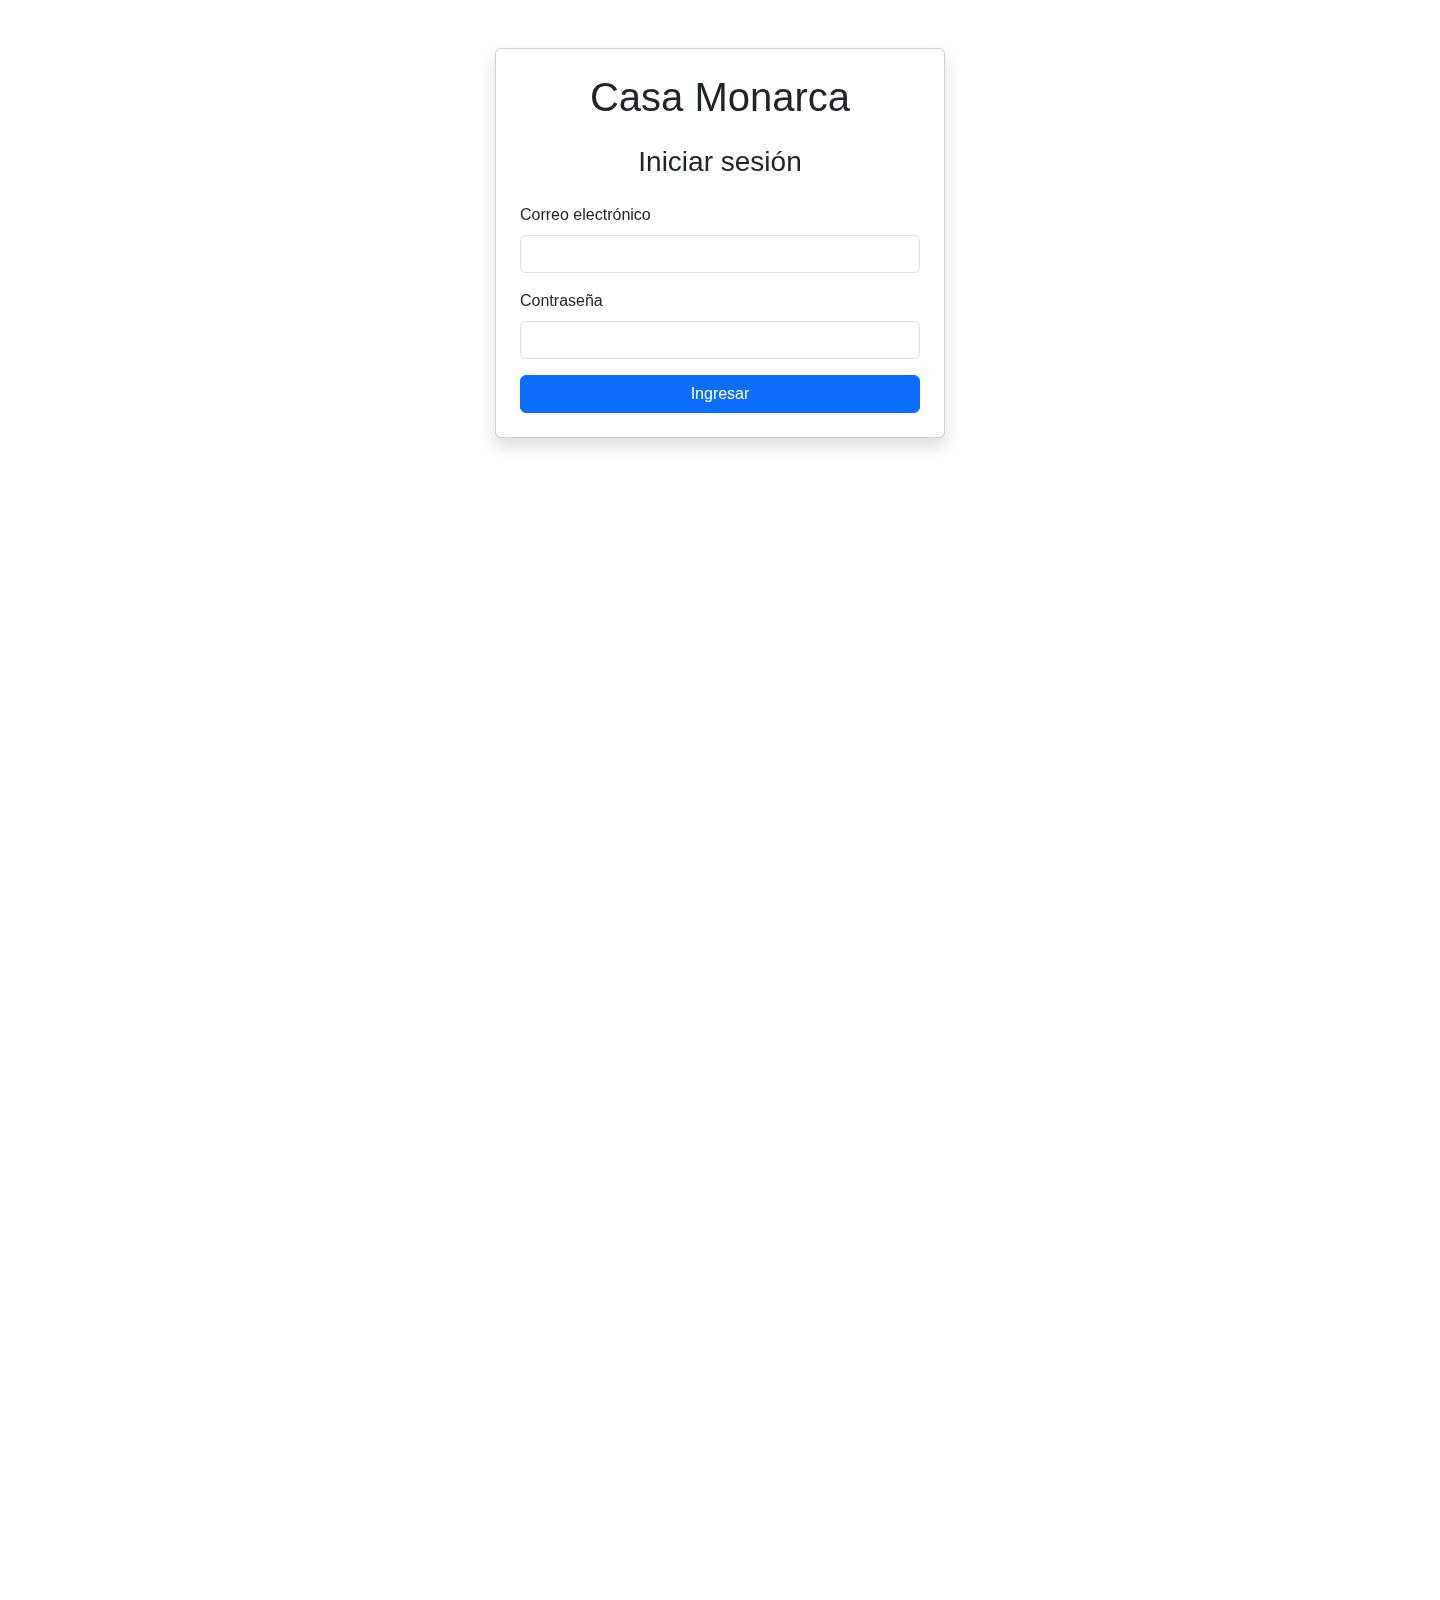
\includegraphics[width=0.78\textwidth]{../manual_usuario/capturas/01-login.png}
\caption{Pantalla de inicio de sesión del Gestor de Identidades y Documentos (elaboración propia).}
\label{fig:login-react}
\end{figure}

\begin{figure}[htbp]
\centering
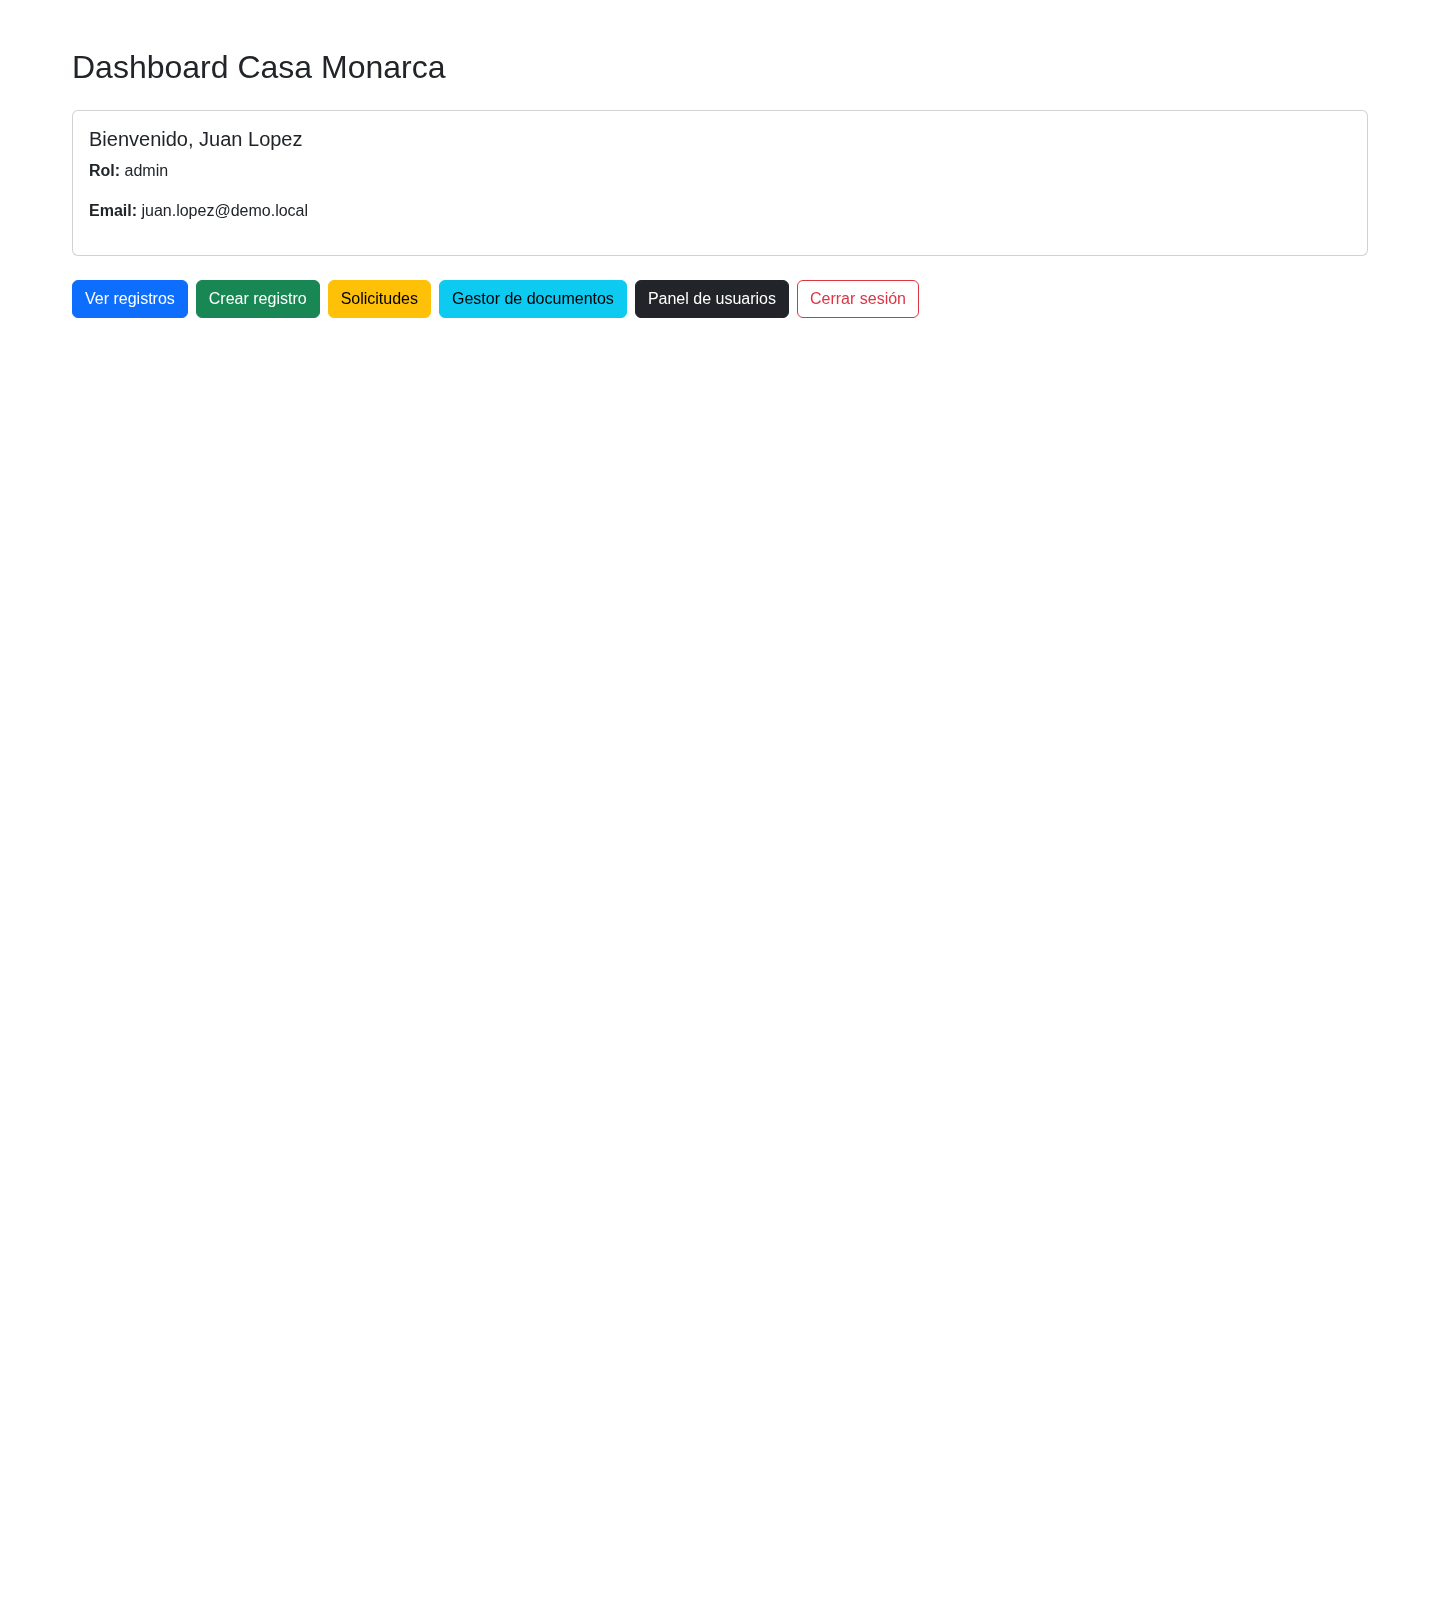
\includegraphics[width=0.78\textwidth]{../manual_usuario/capturas/02-dashboard-admin.png}
\caption{Dashboard del sistema con sesión de administrador iniciada (elaboración propia).}
\label{fig:dashboard-react}
\end{figure}

\section{Desarrollo de Componentes: Backend}
\label{sec:backend}

El backend está compuesto por 22 endpoints PHP independientes ubicados en la carpeta \texttt{api/}. Cada archivo implementa el mismo patrón: lectura de JSON desde \texttt{php://input}, validación de datos, consulta a MySQL mediante \textit{prepared statements} con \texttt{mysqli} y respuesta JSON estructurada con los campos \texttt{success} (booleano) y \texttt{mensaje} (string). Se usa \texttt{ob\_start()} al inicio y \texttt{ob\_clean()} antes de cada respuesta para garantizar JSON puro, sin salida HTML accidental de PHP.

\subsection{Autenticación y control de acceso}
\label{sec:backend-auth}

El endpoint \texttt{login.php} implementa el flujo de autenticación en cuatro verificaciones secuenciales, constituyendo el componente central del módulo de identidades:

\begin{lstlisting}[style=phpstyle, caption={Fragmento de login.php — verificación de credenciales, estado y vigencia (elaboración propia).}]
$stmt = $conexion->prepare(
    "SELECT id, nombre, email, rol, estado,
            fecha_vigencia, certificado_codigo, coordinador_id
     FROM usuarios WHERE email = ?"
);
$stmt->bind_param("s", $email);
$stmt->execute();
$usuario = $stmt->get_result()->fetch_assoc();

// 1. Verificar existencia del usuario
if (!$usuario) {
    echo json_encode(["success" => false,
        "mensaje" => "No existe un usuario con ese correo."]);
    exit;
}
// 2. Verificar estado activo
if ($usuario['estado'] !== 'activo') {
    echo json_encode(["success" => false,
        "mensaje" => "Acceso denegado. El usuario no esta activo."]);
    exit;
}
// 3. Verificar vigencia temporal
if ($usuario['fecha_vigencia'] < date('Y-m-d')) {
    echo json_encode(["success" => false,
        "mensaje" => "Acceso denegado. La vigencia ha expirado."]);
    exit;
}
// 4. Verificar hash BCRYPT
if (!password_verify($password, $usuario['password'])) {
    echo json_encode(["success" => false,
        "mensaje" => "Contrasena incorrecta."]);
    exit;
}
echo json_encode(["success" => true, "usuario" => $usuario]);
\end{lstlisting}

Este flujo garantiza que solo usuarios con estado \texttt{activo} y vigencia futura puedan autenticarse, validando en orden: existencia, estado, vigencia y contraseña. Cada verificación produce un mensaje diferenciado, facilitando el diagnóstico sin exponer información de seguridad innecesaria.

\subsection{Firma digital RSA con OpenSSL}
\label{sec:backend-firma}

El endpoint \texttt{firmar\_documento.php} implementa la firma digital de documentos en cuatro pasos que aplican directamente los conceptos de clave pública estudiados en el bloque:

\begin{lstlisting}[style=phpstyle, caption={Fragmento de firmar\_documento.php — firma RSA-2048 con SHA-256 (elaboración propia).}]
// 1. Obtener clave privada cifrada del coordinador desde MySQL
$clave_privada_cifrada = $usuario['clave_privada_cifrada'];

// 2. Descifrar la clave privada con la contrasena del coordinador
$clave_privada = openssl_pkey_get_private(
    $clave_privada_cifrada,
    $password_firma
);
if (!$clave_privada) {
    echo json_encode(["success" => false,
        "mensaje" => "Contrasena de firma incorrecta."]);
    exit;
}

// 3. Calcular hash SHA-256 del archivo fisico
$hash = hash_file('sha256', $ruta_archivo);

// 4. Firmar el hash con la clave privada RSA-2048
openssl_sign($hash, $firma_raw, $clave_privada, OPENSSL_ALGO_SHA256);
$firma_base64 = base64_encode($firma_raw);

// Generar folio unico y almacenar en MySQL
$folio = "FIR-" . date("Ymd-His")
       . "-DOC{$documento_id}-USR{$usuario_id}";
\end{lstlisting}

La verificación posterior (\texttt{verificar\_firma\_documento.php}) recalcula el hash SHA-256 del archivo físico actual y lo valida contra la firma almacenada usando \texttt{openssl\_verify} con la clave pública del coordinador, detectando cualquier modificación posterior a la firma. La generación de llaves RSA-2048 para los coordinadores se realiza en \texttt{generar\_llaves\_coordinador.php}, almacenando la clave pública en texto PEM y la clave privada cifrada con la contraseña elegida por el coordinador.

\section{Desarrollo de Componentes: Frontend}
\label{sec:frontend}

El frontend es una aplicación de página única (SPA) construida con React~19 y compilada por Vite~8. La navegación entre páginas se gestiona con React Router DOM~7.14, con protección de rutas mediante el componente \texttt{ProtectedRoute.jsx}, que consulta la sesión contra \texttt{/api/validar\_sesion.php} antes de renderizar cada página protegida.

\subsection{Arquitectura de componentes y enrutamiento}

\begin{table}[H]
\centering
\caption{Páginas principales del frontend React y roles autorizados (elaboración propia).}
\label{tab:paginas-react}
\begin{tabular}{p{0.34\textwidth} p{0.20\textwidth} p{0.33\textwidth}}
\toprule
\textbf{Componente} & \textbf{Ruta} & \textbf{Roles permitidos} \\
\midrule
\texttt{Login.jsx} & \texttt{/} & Público \\
\texttt{Dashboard.jsx} & \texttt{/dashboard} & Todos autenticados \\
\texttt{AdminPanel.jsx} & \texttt{/admin} & admin \\
\texttt{GestorDocumentos.jsx} & \texttt{/gestor} & Todos autenticados \\
\texttt{Migrantes.jsx} & \texttt{/migrantes} & Todos autenticados \\
\texttt{CrearMigrante.jsx} & \texttt{/migrantes/crear} & admin, coordinador, operador \\
\texttt{SolicitudesPush.jsx} & \texttt{/solicitudes} & Todos autenticados \\
\bottomrule
\end{tabular}
\end{table}

\subsection{Módulo Gestor de Documentos}

El componente \texttt{GestorDocumentos.jsx} implementa el flujo VOCA completo mediante llamadas \texttt{fetch} asíncronas a los endpoints del backend. La Figura~\ref{fig:gestor-inicial} muestra el estado inicial del módulo con estadísticas por etapa; la Figura~\ref{fig:nuevo-documento} muestra el formulario de registro de un nuevo documento.

\begin{figure}[htbp]
\centering
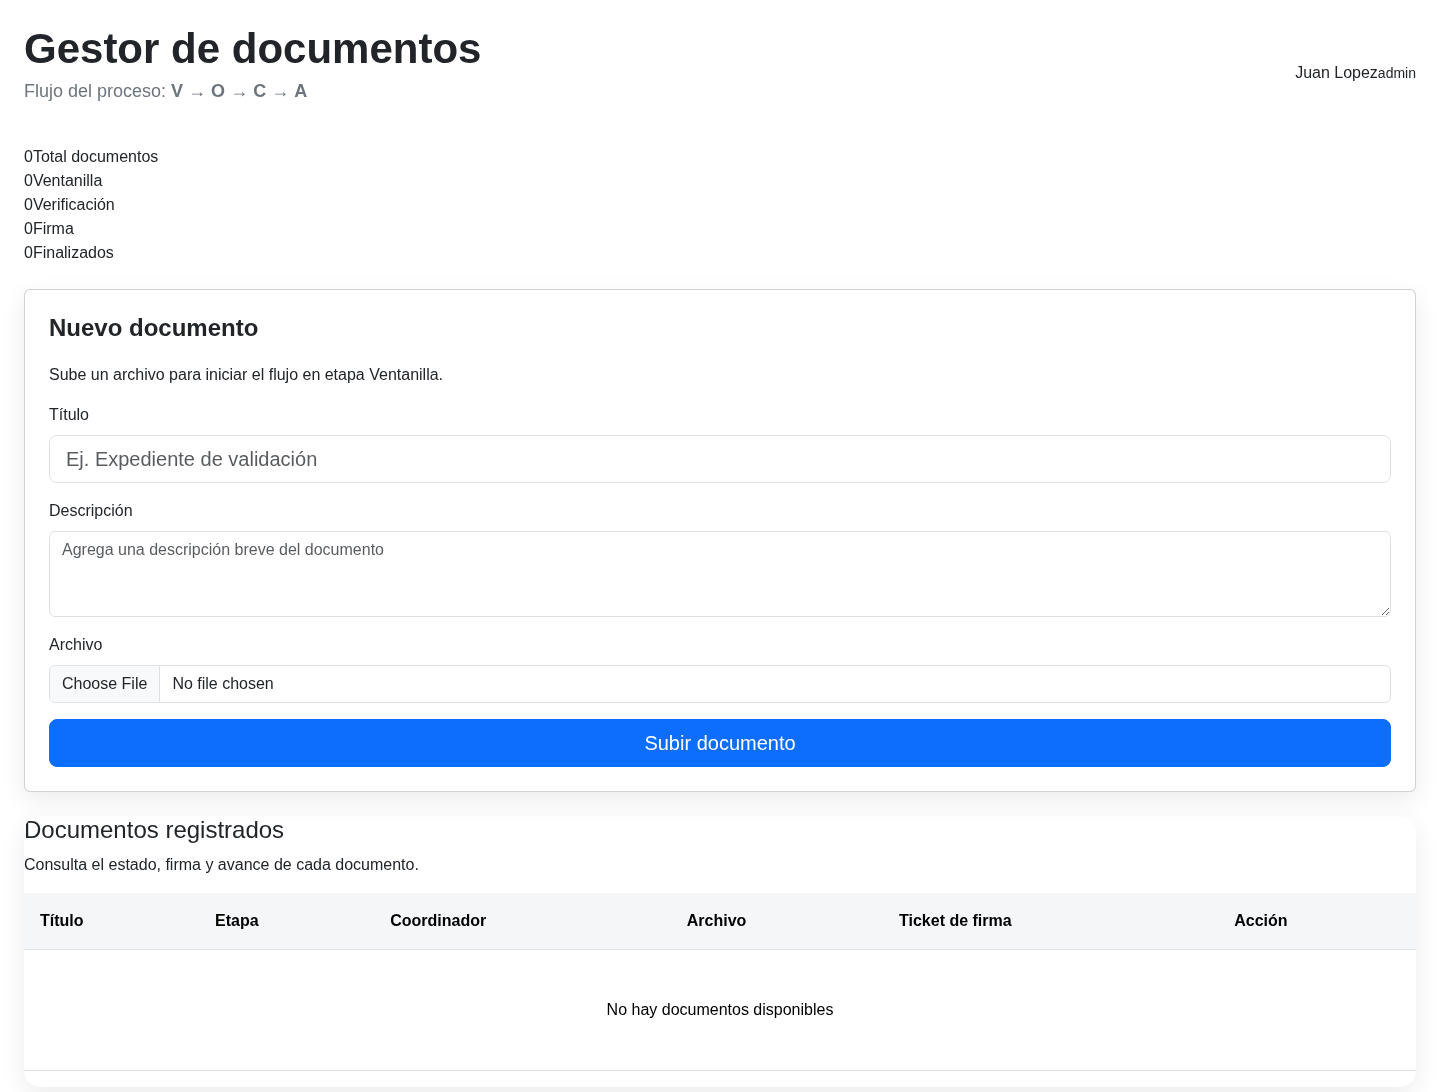
\includegraphics[width=0.75\textwidth]{../manual_usuario/capturas/03-gestor-documentos-inicial.png}
\caption{Vista inicial del Gestor de Documentos con estadísticas por etapa (elaboración propia).}
\label{fig:gestor-inicial}
\end{figure}

\begin{figure}[htbp]
\centering
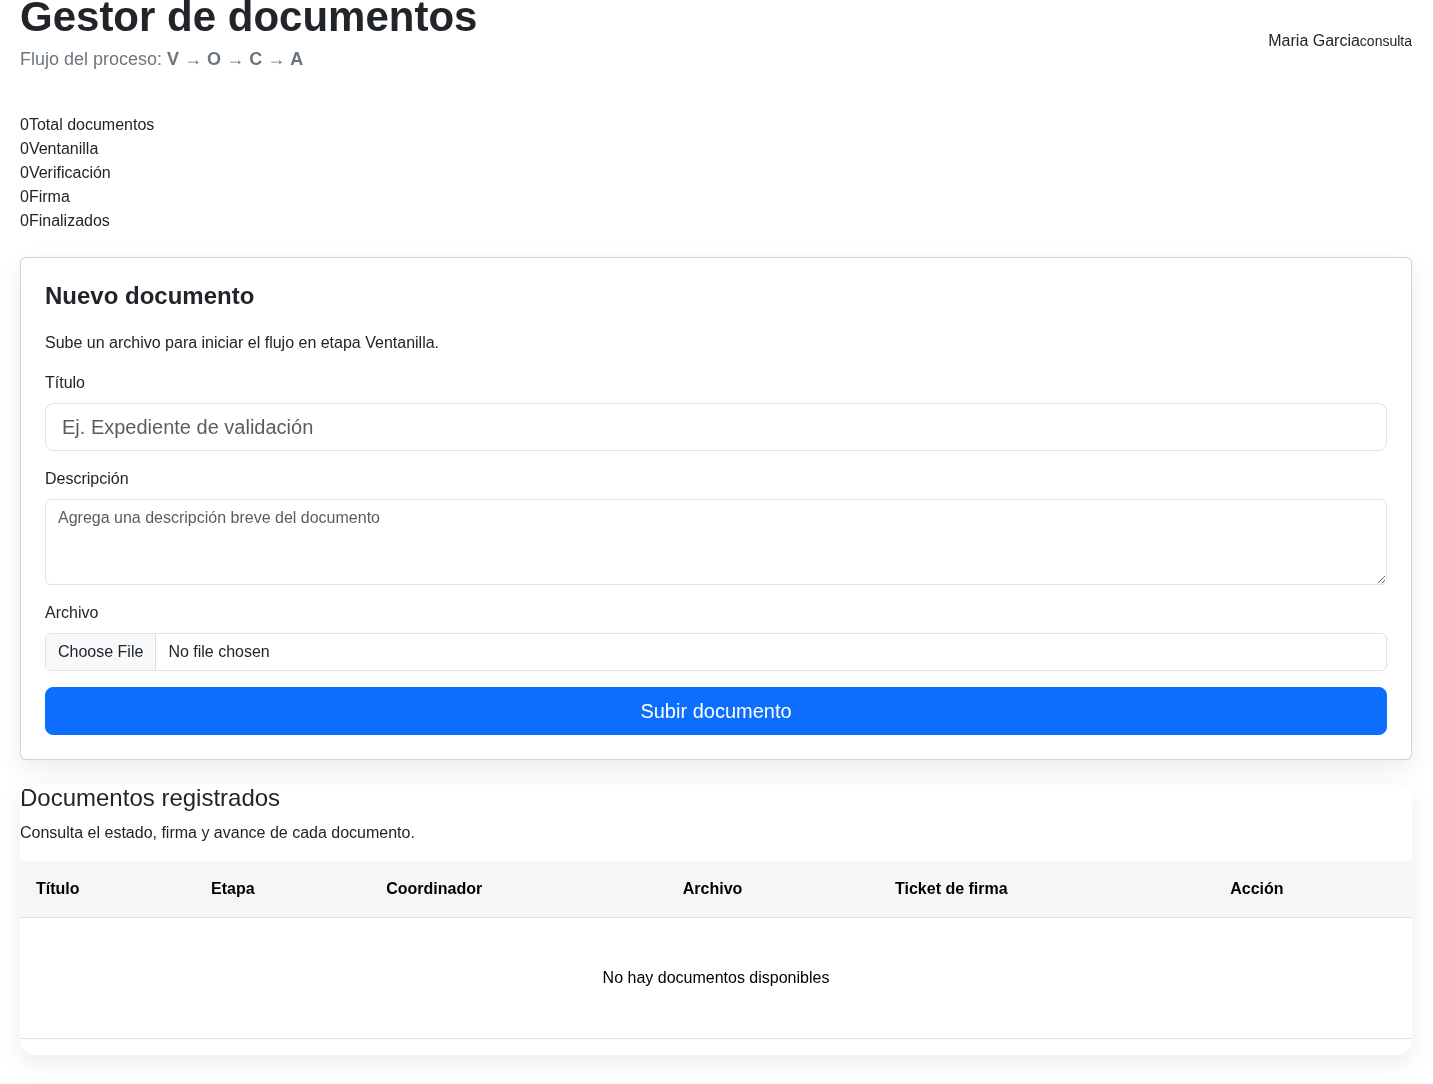
\includegraphics[width=0.78\textwidth]{../manual_usuario/capturas/04-formulario-nuevo-documento.png}
\caption{Formulario de registro de un nuevo documento en etapa Ventanilla (elaboración propia).}
\label{fig:nuevo-documento}
\end{figure}

\subsection{Flujo de firma digital en el frontend}

La Figura~\ref{fig:firma-coordinador} muestra la interfaz de firma digital disponible para el coordinador, y la Figura~\ref{fig:ticket-firma} muestra el ticket de firma generado tras la operación criptográfica.

\begin{figure}[htbp]
\centering
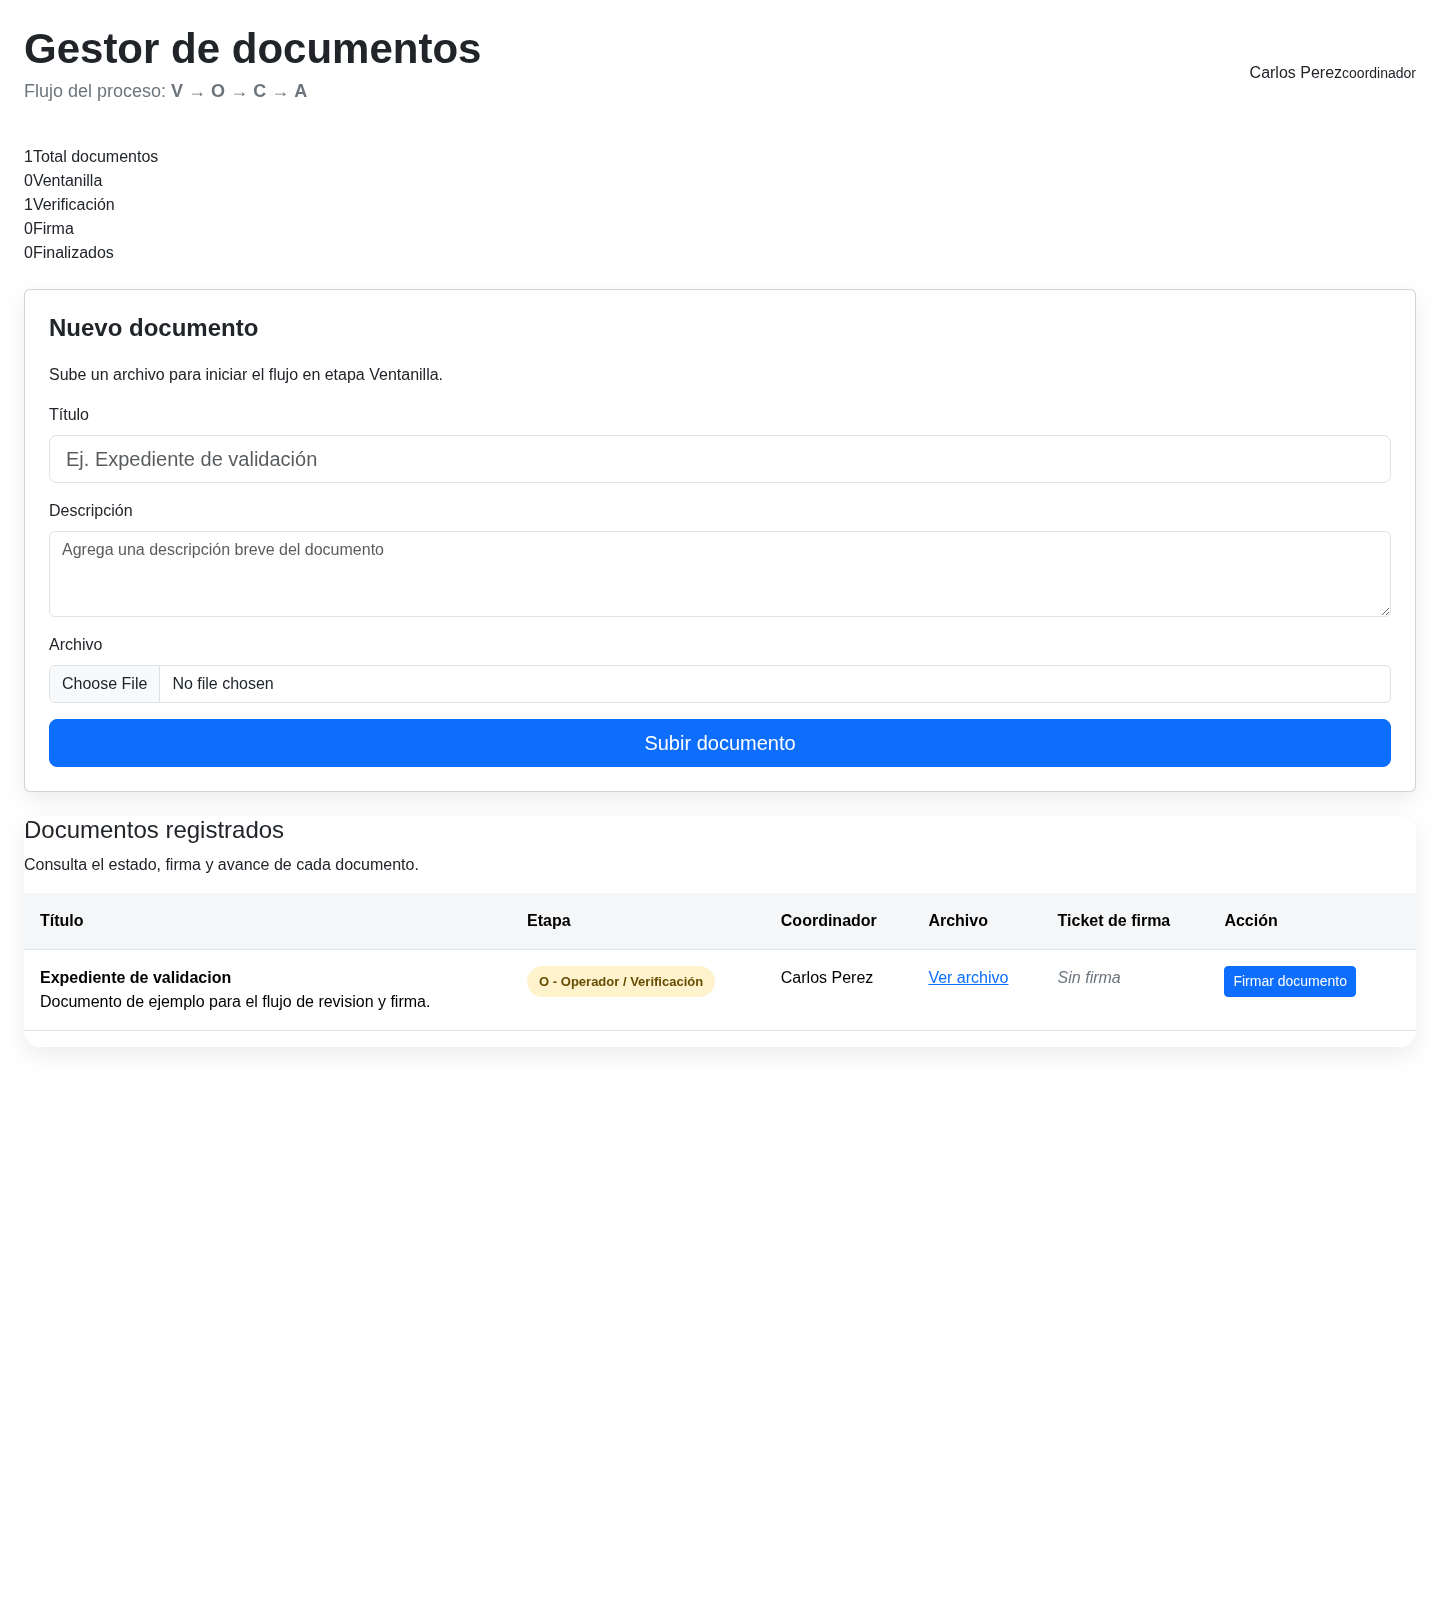
\includegraphics[width=0.78\textwidth]{../manual_usuario/capturas/08-firma-coordinador.png}
\caption{Interfaz de firma digital disponible para el coordinador en etapa Operador (elaboración propia).}
\label{fig:firma-coordinador}
\end{figure}

\begin{figure}[htbp]
\centering
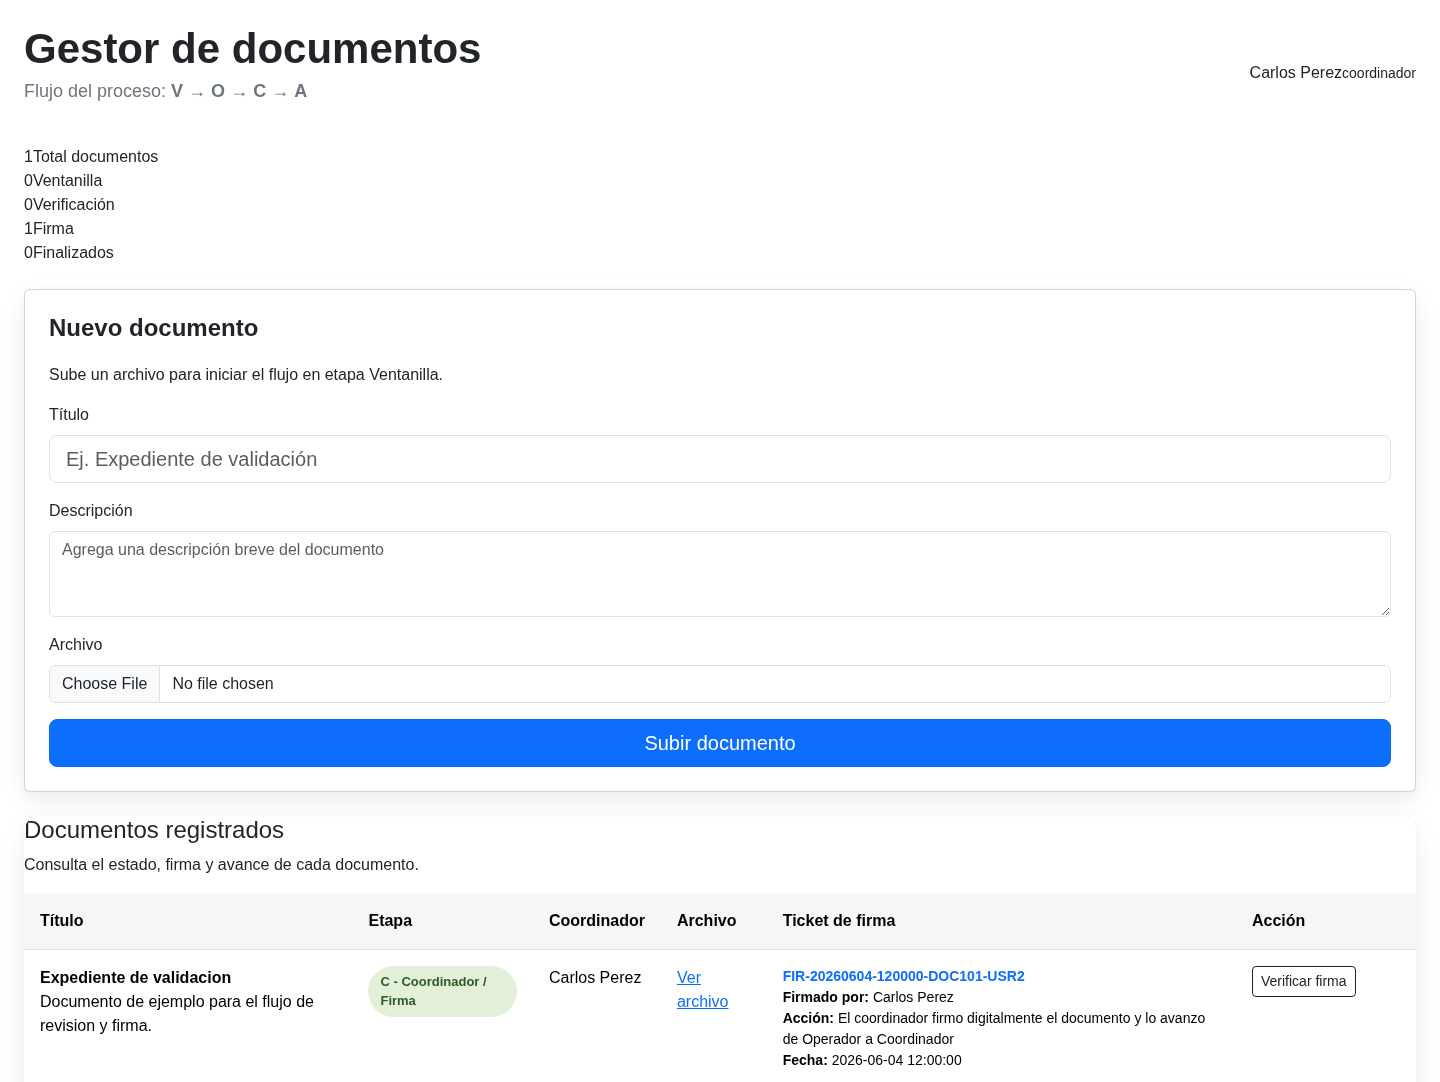
\includegraphics[width=0.78\textwidth]{../manual_usuario/capturas/09-ticket-firma.png}
\caption{Ticket y folio de firma digital generados tras la operación criptográfica (elaboración propia).}
\label{fig:ticket-firma}
\end{figure}

\section{Conexión de los Componentes}
\label{sec:conexion}

La comunicación entre el frontend React y el backend PHP se realiza mediante el proxy de desarrollo de Vite, configurado en \texttt{vite.config.js}:

\begin{lstlisting}[style=jsstyle, caption={Configuración del proxy de desarrollo en vite.config.js (elaboración propia).}]
server: {
  proxy: {
    '/api': {
      target: 'http://localhost',
      changeOrigin: true,
      rewrite: (path) => path
    }
  }
}
\end{lstlisting}

Esta configuración permite que el frontend en \texttt{localhost:5173} realice llamadas a \texttt{/api/*.php} y estas sean redirigidas transparentemente a \texttt{http://localhost/casa-monarca-frontend/api/}, eliminando problemas de CORS durante el desarrollo. En producción, el bundle generado por \texttt{npm run build} se sirve directamente desde Apache en el mismo dominio que los endpoints PHP.

El flujo completo de una operación representativa —la firma digital de un documento— ilustra la integración de las tres capas:

\begin{enumerate}[label=\arabic*.]
  \item El coordinador presiona \textbf{Firmar documento} en \texttt{GestorDocumentos.jsx} e ingresa su contraseña de firma.
  \item React realiza un \texttt{fetch POST} a \texttt{/api/firmar\_documento.php} con \texttt{documento\_id}, \texttt{usuario\_id} y \texttt{password\_firma} en formato JSON.
  \item Vite redirige la petición a Apache, que enruta al archivo PHP correspondiente.
  \item PHP recupera la clave privada cifrada de MySQL, la descifra con la contraseña, calcula el hash SHA-256 del archivo físico y firma con \texttt{openssl\_sign} (RSA-2048).
  \item La firma en Base64 y el folio único se almacenan en MySQL; la respuesta JSON incluye \texttt{etapa: "C"}, el folio y los coordinadores adicionales pendientes.
  \item React actualiza el estado del componente y muestra el ticket de firma al coordinador.
\end{enumerate}

%%============================================================
%% CAPÍTULO 4 — RESULTADOS
%%============================================================
\chapter{Resultados}

\section{Resultados del Backend}

Los 22 endpoints del backend respondieron correctamente en todos los escenarios de prueba. Los resultados más relevantes son:

\begin{itemize}
  \item \textbf{Autenticación}: \texttt{login.php} rechaza correctamente usuarios eliminados, inactivos, revocados y con vigencia vencida, emitiendo mensajes diferenciados para cada caso, sin exponer información de la base de datos.
  \item \textbf{Control de acceso por rol}: la validación de rol en cada endpoint impide que usuarios sin privilegios ejecuten operaciones administrativas, incluso si construyen manualmente la petición HTTP.
  \item \textbf{Firma digital}: \texttt{firmar\_documento.php} genera firmas RSA-2048 válidas verificables por \texttt{verificar\_firma\_documento.php}. La integridad del archivo se confirma al recalcular SHA-256 en cada verificación, detectando cualquier modificación posterior.
  \item \textbf{Generación de llaves RSA}: \texttt{generar\_llaves\_coordinador.php} genera pares de llaves RSA-2048 con OpenSSL, almacenando la clave pública en PEM y la clave privada cifrada con la contraseña del coordinador.
  \item \textbf{Persistencia}: las operaciones CRUD sobre usuarios, documentos, migrantes y solicitudes se persisten en MySQL con prepared statements, sin vulnerabilidades de inyección SQL.
\end{itemize}

\section{Resultados del Frontend}

La interfaz React implementa correctamente el flujo completo del sistema:

\begin{itemize}
  \item El login redirige al dashboard diferenciado por rol; las rutas protegidas bloquean el acceso a páginas no autorizadas.
  \item El Gestor de Documentos muestra estadísticas por etapa y permite ejecutar todas las acciones del flujo VOCA según el rol del usuario en sesión.
  \item La firma digital se ejecuta desde el frontend ingresando la contraseña; el ticket resultante se muestra inmediatamente al coordinador.
  \item La verificación de integridad es accesible para todos los roles y confirma si la firma almacenada corresponde al archivo actual.
\end{itemize}

La Figura~\ref{fig:verificacion} muestra la verificación de integridad de un documento firmado; la Figura~\ref{fig:documento-finalizado} muestra un documento completado en la etapa de Inserción final.

\begin{figure}[htbp]
\centering
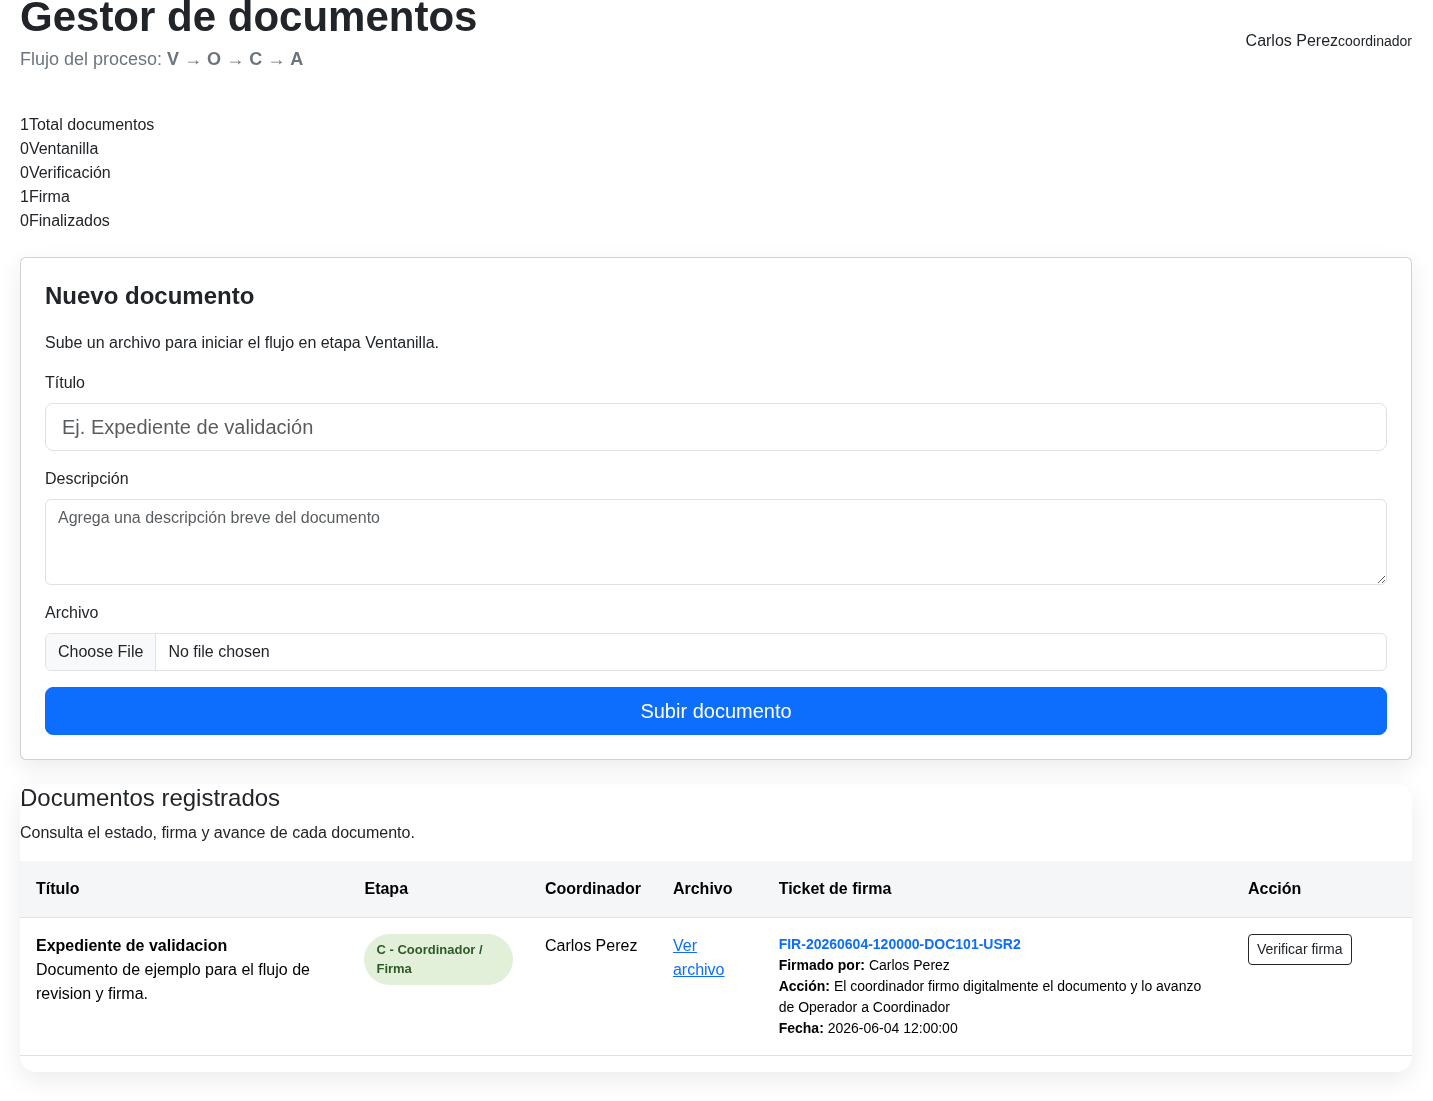
\includegraphics[width=0.78\textwidth]{../manual_usuario/capturas/10-verificacion-firma.png}
\caption{Verificación de firma digital: el sistema confirma la integridad del documento (elaboración propia).}
\label{fig:verificacion}
\end{figure}

\begin{figure}[htbp]
\centering
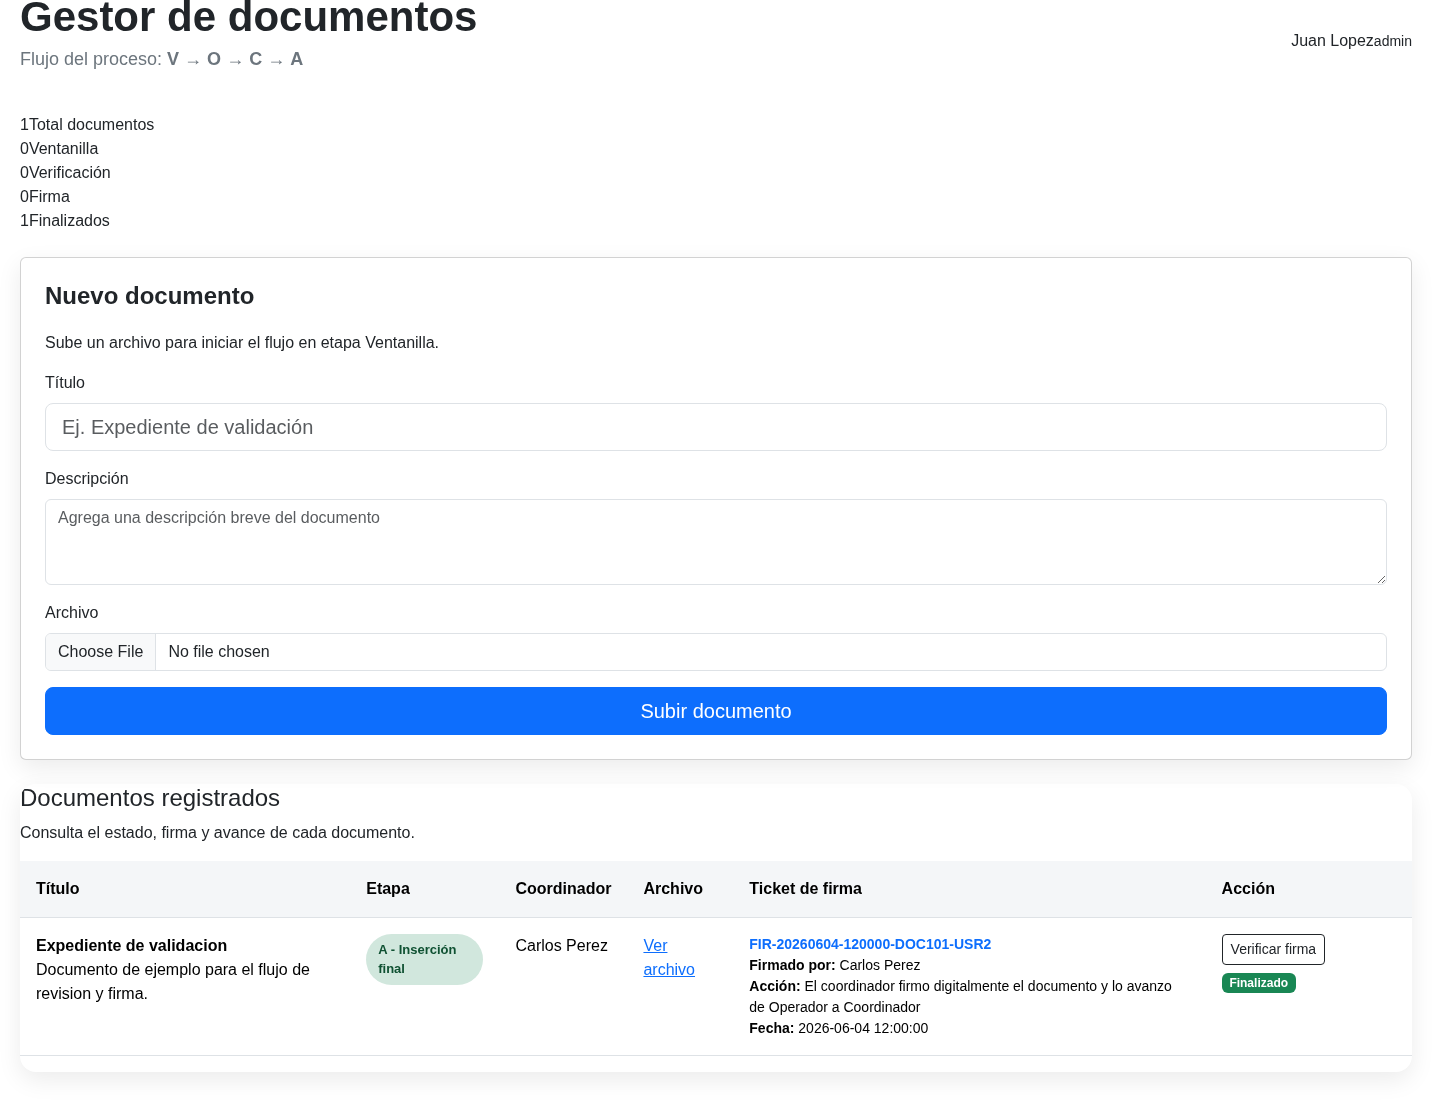
\includegraphics[width=0.78\textwidth]{../manual_usuario/capturas/12-documento-finalizado.png}
\caption{Documento completado en etapa de Inserción Final tras recorrer el flujo VOCA completo (elaboración propia).}
\label{fig:documento-finalizado}
\end{figure}

\section{Resultados de la Solución Completa}

La solución integra de manera funcional el módulo de identidades (autenticación, RBAC, certificados, vigencias) con el módulo documental (flujo VOCA, firma RSA, verificación SHA-256) y los módulos operativos (registro de migrantes, solicitudes push). El flujo completo de un documento —desde su carga en Ventanilla hasta la Inserción final— opera sin intervención manual fuera del sistema y deja trazabilidad completa en la tabla \texttt{documentos\_historial}, que registra cada cambio de etapa con el usuario responsable, la fecha y un comentario asociado.

\section{Casos de Uso y Tabla de Validaciones}
\label{sec:validaciones}

Se ejecutaron 15 casos de prueba de caja negra sobre los módulos de identidad y control de acceso. La metodología consistió en definir precondiciones específicas, ejecutar la acción y verificar que la respuesta del sistema coincidiera con el resultado esperado. La Tabla~\ref{tab:validaciones} resume los resultados con referencia a la evidencia recolectada.

\begin{longtable}{p{0.04\textwidth} p{0.25\textwidth} p{0.25\textwidth} p{0.24\textwidth} p{0.09\textwidth}}
\caption{Matriz de validación y casos de uso del Gestor de Identidades y Documentos (elaboración propia).}
\label{tab:validaciones}\\
\toprule
\textbf{ID} & \textbf{Descripción} & \textbf{Resultado esperado} & \textbf{Evidencia} & \textbf{Status} \\
\midrule
\endfirsthead
\toprule
\textbf{ID} & \textbf{Descripción} & \textbf{Resultado esperado} & \textbf{Evidencia} & \textbf{Status} \\
\midrule
\endhead
1 & Inicio de sesión correcto con usuario administrador. &
  Redireccionamiento al dashboard; nombre y rol visibles. &
  \hyperref[fig:login-react]{Fig.~\ref*{fig:login-react}}, \hyperref[fig:dashboard-react]{Fig.~\ref*{fig:dashboard-react}} &
  \textcolor{passgreen}{\textbf{Pass}} \\
\midrule
2 & Acceso del administrador al panel de administración. &
  Panel de usuarios cargado; botones de crear, editar y eliminar visibles. &
  \hyperref[fig:dashboard-react]{Fig.~\ref*{fig:dashboard-react}}, Anexo~\ref{anx:diccionario} &
  \textcolor{passgreen}{\textbf{Pass}} \\
\midrule
3 & Usuario sin rol admin intenta acceder al panel de administración. &
  Acceso denegado; redirección al login. &
  \hyperref[fig:login-react]{Fig.~\ref*{fig:login-react}}, \hyperref[sec:backend-auth]{Secc.~\ref*{sec:backend-auth}} &
  \textcolor{passgreen}{\textbf{Pass}} \\
\midrule
4 & Creación de usuario por administrador con generación automática de certificado. &
  Usuario guardado; \texttt{certificado\_codigo}, \texttt{estado} y \texttt{fecha\_vigencia} generados. &
  Anexo~\ref{anx:diccionario}, \hyperref[sec:backend-auth]{Secc.~\ref*{sec:backend-auth}} &
  \textcolor{passgreen}{\textbf{Pass}} \\
\midrule
5 & Edición de usuario por administrador. &
  Datos actualizados en la BD y reflejados en el panel. &
  \hyperref[sec:backend-auth]{Secc.~\ref*{sec:backend-auth}} &
  \textcolor{passgreen}{\textbf{Pass}} \\
\midrule
6 & Eliminación de usuario por administrador. &
  Usuario eliminado de la tabla; ya no aparece en el panel. &
  \hyperref[sec:backend-auth]{Secc.~\ref*{sec:backend-auth}} &
  \textcolor{passgreen}{\textbf{Pass}} \\
\midrule
7 & Usuario eliminado intenta iniciar sesión. &
  Sistema rechaza con: \textit{No existe un usuario con ese correo.} &
  \hyperref[sec:backend-auth]{Secc.~\ref*{sec:backend-auth}}, Lst.~4.1 &
  \textcolor{passgreen}{\textbf{Pass}} \\
\midrule
8 & Usuario activo y vigente puede iniciar sesión. &
  Acceso permitido; dashboard visible con rol correcto. &
  \hyperref[fig:login-react]{Fig.~\ref*{fig:login-react}}, \hyperref[fig:dashboard-react]{Fig.~\ref*{fig:dashboard-react}} &
  \textcolor{passgreen}{\textbf{Pass}} \\
\midrule
9 & Usuario inactivo intenta iniciar sesión. &
  Sistema rechaza con: \textit{Acceso denegado. El usuario no está activo.} &
  \hyperref[sec:backend-auth]{Secc.~\ref*{sec:backend-auth}}, Lst.~4.1 &
  \textcolor{passgreen}{\textbf{Pass}} \\
\midrule
10 & Usuario revocado intenta iniciar sesión. &
  Sistema rechaza con: \textit{Acceso denegado. El usuario no está activo.} &
  \hyperref[sec:backend-auth]{Secc.~\ref*{sec:backend-auth}}, Lst.~4.1 &
  \textcolor{passgreen}{\textbf{Pass}} \\
\midrule
11 & Usuario con vigencia vencida intenta iniciar sesión. &
  Sistema rechaza con: \textit{Acceso denegado. La vigencia ha expirado.} &
  \hyperref[sec:backend-auth]{Secc.~\ref*{sec:backend-auth}}, Lst.~4.1 &
  \textcolor{passgreen}{\textbf{Pass}} \\
\midrule
12 & Intento de inicio de sesión con contraseña incorrecta. &
  Sistema rechaza con: \textit{Contraseña incorrecta.} &
  \hyperref[sec:backend-auth]{Secc.~\ref*{sec:backend-auth}}, Lst.~4.1 &
  \textcolor{passgreen}{\textbf{Pass}} \\
\midrule
13 & Correo no registrado intenta iniciar sesión. &
  Sistema rechaza con: \textit{No existe un usuario con ese correo.} &
  \hyperref[sec:backend-auth]{Secc.~\ref*{sec:backend-auth}}, Lst.~4.1 &
  \textcolor{passgreen}{\textbf{Pass}} \\
\midrule
14 & Persistencia de datos de certificado al crear usuario. &
  Campos \texttt{estado}, \texttt{fecha\_vigencia} y \texttt{certificado\_codigo} con valores válidos en MySQL. &
  Anexo~\ref{anx:diccionario} &
  \textcolor{passgreen}{\textbf{Pass}} \\
\midrule
15 & Restricción de privilegios para usuario no administrador en operaciones CRUD. &
  Sistema bloquea crear, editar o eliminar usuarios si el rol no es admin. &
  \hyperref[fig:dashboard-react]{Fig.~\ref*{fig:dashboard-react}}, \hyperref[sec:backend-auth]{Secc.~\ref*{sec:backend-auth}} &
  \textcolor{passgreen}{\textbf{Pass}} \\
\bottomrule
\end{longtable}

%%============================================================
%% CAPÍTULO 5 — CONCLUSIONES Y TRABAJO FUTURO
%%============================================================
\chapter{Conclusiones y Trabajo Futuro}

\section{Conclusiones}

La implementación del Gestor de Identidades y Documentos para Casa Monarca demostró que es posible construir un sistema de control de acceso con fundamentos criptográficos sólidos sobre un stack tecnológico accesible (React + PHP + MySQL), sin depender de infraestructura costosa en la nube y con una curva de mantenimiento adecuada para el personal interno de una ONG.

Los 15 casos de prueba de caja negra sobre el módulo de autenticación y control de acceso confirman que el sistema cumple con los objetivos planteados: solo usuarios con estado \texttt{activo}, vigencia futura y credenciales correctas pueden autenticarse; las operaciones administrativas están restringidas al rol correspondiente tanto en el frontend (rutas protegidas) como en el backend (validación en cada endpoint); y los certificados digitales únicos generados automáticamente por usuario proveen una base de identidad verificable.

La extensión del alcance hacia la firma digital de documentos con RSA-2048 y SHA-256 aplicó directamente los conceptos estudiados en el bloque: las recomendaciones del NIST SP 800-56B para la fortaleza de pares de llaves, la entropía de Shannon para la aleatoriedad de certificados y el modelo de confianza del SAT para la arquitectura de roles y custodia de llaves privadas. Este módulo responde a una necesidad real del socio formador de contar con un mecanismo objetivamente verificable para la autorización de documentos institucionales.

Desde una perspectiva de seguridad informática, el uso de BCRYPT para el hash de contraseñas, de prepared statements para prevenir inyección SQL (OWASP Top 10) y de OpenSSL para la generación y gestión de llaves asimétricas establece una base criptográfica sólida sobre la que pueden construirse versiones futuras del sistema.

\section{Trabajo Futuro}

\begin{itemize}
  \item \textbf{Plan de pruebas extendido}: diseñar casos de prueba formales para los módulos de firma digital, migrantes y solicitudes push, que actualmente operan pero no cuentan con una matriz de validación documentada.
  \item \textbf{Pruebas de aceptación}: realizar pruebas con el socio formador en el entorno de producción (HostGator), verificando en particular la disponibilidad y configuración de la extensión OpenSSL en el servidor de hospedaje.
  \item \textbf{Gestión de sesión}: migrar el almacenamiento de sesión de \texttt{localStorage} a tokens JWT con cookies \texttt{HttpOnly} para reducir la superficie de ataque ante XSS.
  \item \textbf{Política CORS}: unificar y restringir los headers \texttt{Access-Control-Allow-Origin} a dominios específicos en producción, en lugar del comodín \texttt{*} utilizado durante el desarrollo.
  \item \textbf{Panel de auditoría}: aprovechar la tabla \texttt{documentos\_historial} para construir un módulo de trazabilidad que muestre el historial completo de cambios de etapa de cada documento, con el usuario responsable y la fecha.
  \item \textbf{Notificaciones}: implementar alertas automáticas de vencimiento próximo de certificado o vigencia de usuario, para reducir la carga administrativa del equipo de Casa Monarca.
  \item \textbf{Paginación}: implementar paginación en las tablas de documentos, migrantes y usuarios para garantizar la escalabilidad del sistema conforme crezca el volumen de registros.
\end{itemize}

%%============================================================
%% REFERENCIAS
%%============================================================
\chapter*{Referencias}
\addcontentsline{toc}{chapter}{Referencias}

\begin{enumerate}[label={[\arabic*]}]
  \item Ramió Aguirre, J. (2006). \textit{Libro electrónico de seguridad informática y criptografía} (Versión 4.1). Universidad Politécnica de Madrid.

  \item Barker, E., Chen, L., Roginsky, A., Vassilev, A., Davis, R., \& Simon, S. (2019). \textit{NIST Special Publication 800-56B Revision 2: Recommendation for pair-wise key establishment using integer factorization cryptography}. National Institute of Standards and Technology, U.S. Department of Commerce.

  \item Shannon, C. E. (2001). A mathematical theory of communication. \textit{ACM SIGMOBILE Mobile Computing and Communications Review}, \textit{5}(1), 3--55.

  \item The PHP Group. (s.f.). \textit{OpenSSL functions}. PHP Manual. \url{https://www.php.net/manual/es/book.openssl.php}

  \item The PHP Group. (s.f.). \textit{mysqli prepared statements}. PHP Manual. \url{https://www.php.net/manual/es/class.mysqli.php}

  \item React. (2024). \textit{React: The library for web and native user interfaces}. \url{https://react.dev}

  \item Vite. (2024). \textit{Vite: Next generation frontend tooling}. \url{https://vite.dev}

  \item Casa Monarca, Ayuda Humanitaria al Migrante, A.B.P. (s.f.). \textit{Sitio web oficial}. \url{https://casamonarca.org.mx/}
\end{enumerate}

%%============================================================
%% ANEXOS
%%============================================================
\appendix

\chapter{Diccionario de Datos — Tabla \texttt{usuarios}}
\label{anx:diccionario}

A continuación se detalla la estructura de la tabla \texttt{usuarios}, que es el eje central del módulo de control de acceso basado en roles (RBAC). Esta tabla centraliza la identidad digital de cada colaborador de Casa Monarca, incluyendo los campos criptográficos necesarios para la firma digital de documentos por parte de los coordinadores.

\begin{table}[H]
\centering
\caption{Diccionario de datos — tabla \texttt{usuarios} (elaboración propia).}
\label{tab:diccionario}
\begin{tabular}{p{0.28\textwidth} p{0.18\textwidth} p{0.43\textwidth}}
\toprule
\textbf{Campo} & \textbf{Tipo SQL} & \textbf{Descripción} \\
\midrule
\texttt{id} & INT AUTO\_INCREMENT & Llave primaria. Identificador único del usuario. \\
\texttt{nombre} & VARCHAR(255) & Nombre oficial registrado en el sistema. \\
\texttt{email} & VARCHAR(255) UNIQUE & Correo electrónico; identificador único de inicio de sesión. \\
\texttt{password} & VARCHAR(255) & Hash BCRYPT de la contraseña. Nunca se almacena en texto plano. \\
\texttt{rol} & VARCHAR(50) & Nivel de privilegios: \texttt{admin}, \texttt{coordinador}, \texttt{operador} o \texttt{consulta}. \\
\texttt{estado} & VARCHAR(50) & Estado de la cuenta: \texttt{activo}, \texttt{inactivo} o \texttt{revocado}. \\
\texttt{fecha\_vigencia} & DATE & Caducidad temporal de la cuenta. Comparada con la fecha actual en cada autenticación. \\
\texttt{certificado\_codigo} & VARCHAR(100) & Código único generado aleatoriamente al crear el usuario. Identidad digital verificable. \\
\texttt{coordinador\_id} & INT & FK lógica a \texttt{usuarios.id}. Define el coordinador asignado a operadores y consultas. \\
\texttt{clave\_publica} & TEXT & Clave pública RSA del coordinador en formato PEM. \\
\texttt{clave\_privada\_cifrada} & TEXT & Clave privada RSA cifrada con la contraseña de firma del coordinador. \\
\bottomrule
\end{tabular}
\end{table}

\chapter{Fragmento de Código — Verificación Criptográfica de Firma}
\label{anx:codigo}

El siguiente fragmento corresponde al endpoint \texttt{verificar\_firma\_documento.php}, que implementa la verificación de integridad de un documento firmado digitalmente. Este proceso recalcula el hash SHA-256 del archivo físico actual y lo valida contra la firma RSA almacenada usando la clave pública del coordinador firmante.

\begin{lstlisting}[style=phpstyle, caption={verificar\_firma\_documento.php — verificación de integridad RSA/SHA-256 (elaboración propia).}]
<?php
ob_start();
header("Access-Control-Allow-Origin: *");
header("Content-Type: application/json");
require_once '../conexion.php';

$data = json_decode(file_get_contents("php://input"), true);
$documento_id = $data['documento_id'] ?? null;

// Obtener documento y clave publica del coordinador
$stmt = $conexion->prepare(
    "SELECT d.firma_coordinador, d.hash_archivo,
            d.archivo_ruta, u.clave_publica
     FROM documentos d
     JOIN usuarios u ON d.firmado_por = u.id
     WHERE d.id = ?"
);
$stmt->bind_param("i", $documento_id);
$stmt->execute();
$row = $stmt->get_result()->fetch_assoc();

// Recalcular hash SHA-256 del archivo fisico actual
$hash_actual = hash_file('sha256', $row['archivo_ruta']);

// Decodificar firma almacenada en Base64
$firma_raw = base64_decode($row['firma_coordinador']);

// Verificar firma RSA con la clave publica del coordinador
$clave_publica = openssl_pkey_get_public($row['clave_publica']);
$resultado = openssl_verify(
    $hash_actual,
    $firma_raw,
    $clave_publica,
    OPENSSL_ALGO_SHA256
);

ob_clean();
if ($resultado === 1) {
    echo json_encode([
        "success"  => true,
        "valida"   => true,
        "mensaje"  => "Firma digital valida. El documento no ha sido modificado."
    ]);
} else {
    echo json_encode([
        "success"  => true,
        "valida"   => false,
        "mensaje"  => "Firma invalida o documento modificado."
    ]);
}
?>
\end{lstlisting}

\end{document}
